\documentclass[a4paper,12pt]{book}
\usepackage[utf8]{inputenc}
\usepackage{graphicx}
\usepackage{epstopdf}
\usepackage{lineno,hyperref}
\usepackage{siunitx}

% The amssymb package provides various useful mathematical symbols
\usepackage{amssymb}
% The amsthm package provides extended theorem environments
\usepackage{amsthm}
\usepackage{amsmath}
\usepackage{amsfonts}
\usepackage{textcomp}

\newcommand{\bs}{\boldsymbol}
\newcommand{\bm}{\mathbf}
\newcommand{\tr}{\mathop{\rm tr }}



\begin{document}

\author{The Vitaproject Team}
\title{Vitaproject Reference Guide}
\date{December 2019}

\frontmatter
\vbox{

	\centering

	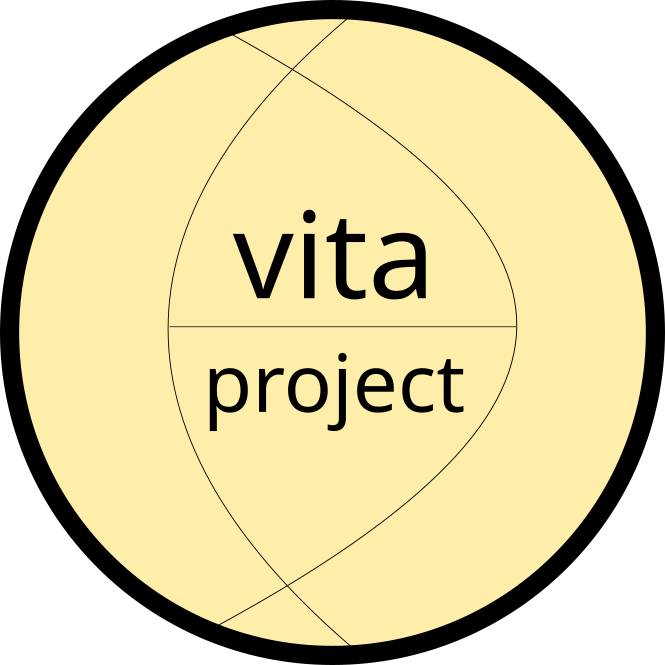
\includegraphics[width=0.4\textwidth]{images/logo}

	\maketitle %this typesets the contents of \title, \author and \date

}
\tableofcontents

\mainmatter
\chapter{Description}

\section{Introduction and functionality}
Vitaproject is part of a comprehensive tool-set for divertor modeling. The function and objectives of each tool, as shown in Figure \ref{fig:scheme}, vary depending on the operating phase. Vitaproject aims to deliver the following functionality:
\begin{description}
	\item [Design, assessment and preparation for operations:] The objective of the modeling in this stage is to have a good estimate of the plasma loading effect, in order to assess compliance to the Design Criteria and to define the Operating Limits. The uncertainty at this stage is large so a large number of sensitivity analysis shall be required in order to establish the range of acceptable plasma parameters, as well as the risk of non-compliance.
%	\item [Pulse monitoring:] validated 2D nonlinear diffusion models are used for real-time temperature estimation. This synthetic diagnostic complements other protection measures such as thermography and thermocouple measurements.
	\item [Post-pulse processing:] A Virtual Thermal Map (VTM) may be used based on processing protection IR camera data. A backup for recreating the surface and bulk temperatures shall be provided through quick analysis of hidden components, cross checking the VTM in case of dubious hotspots, and overall analysis in the case of IR camera malfunctioning.
	\item [Sensitivity, condition and change request assessment:] any change on divertor components may be checked to actual experimental conditions, in order to evaluate the impact of any deviation from nominal geometry and properties as well as to assess major design modifications. This stage differs from the first one in that the model will have been already validated under nominal conditions and the workflow uses experimental data.
\end{description}

The workflow implemented bridges the Physics design, operational database and the engineering design and assessment.

\begin{figure*}[htbp]
	\centering
	%  \vspace{-15mm}
	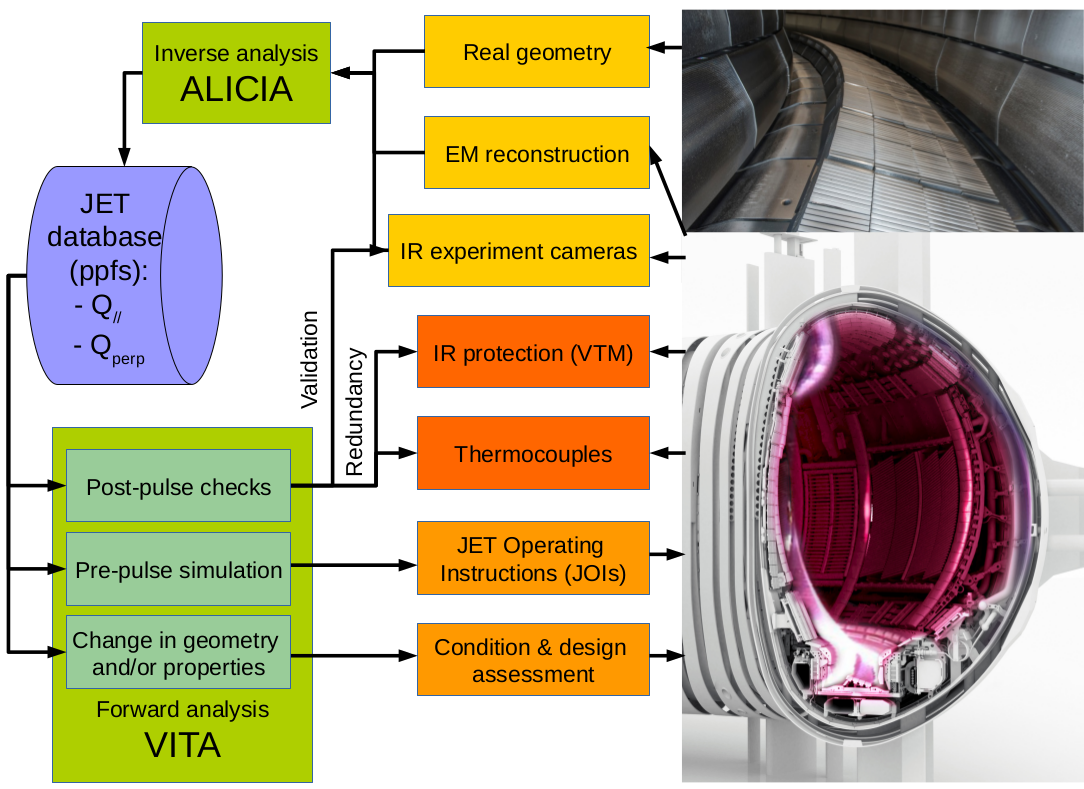
\includegraphics[width=0.90\linewidth]{images/scheme_software}
	\caption{Overall workflow scheme}
	\label{fig:scheme}
\end{figure*}


\section{Description}
\textit{Virtual Thermal Assessments} is a forward simulation code featuring a GUI
%---shown in Figure \ref{fig:vita}---
for ease of use. Its main goal is to allow both quick and accurate analysis of divertor tiles to users by setting global machine parameters, recreating previous stored pulses, or a mix of both. The time varying boundary conditions and integration parameters are automatically set, therefore not requiring the user to deal with numerical details.

It is designed for design, pulse preparation activities, post-pulse checks, and integrity assessments of in-vessel components. It may also be used to test alternative divertor configurations under experimental conditions. It includes the following capabilities:
\begin{itemize}
	\item Several ways for defining pulse parameters and automatically setting the simulation model and its boundary conditions.
	\item Connection to the experimental database for the readout of diagnostic measurements, typically temperatures.
	\item Selection of the wall segment or divertor tile with different accuracy on the thermal model.
	\item Direct plotting of diagnostic synthetic signals.
	\item Tabulated output of maximum temperature at the surface and thermocouple measurement locations, along with energy values.
\end{itemize}

The parameters that define the pulse can be grouped as follows:
\begin{description}
	\item [Input power parameters:] The total power input to the plasma arrives from either resistive heating, NBI or RF sources. Each of the three signals can be defined as a constant value or a table from a file allowing complex manual load inputs. In the case where an experimental pulse is to be recreated, each of these values can be read from their corresponding signal in the JET database.
	\item [Plasma parameters:] The total power arriving to the divertor at any moment in time corresponds to the total minus the radiated power. This is taken into account as a factor in the range $[0-1]$ called the radiated fraction. The outboard-inboard power ratio is typically estimated in single null configurations as $1/3$ inboard, $2/3$ outboard, and $1/10$ inboard, $9/10$ outboard in double null configurations. The footprint can be defined using different functions:
	\begin{itemize}
		\item A pure exponential function is the simplest way of defining the shape of the SOL power density around the plasma. When information about the far-SOL is known, a double exponential function may be used. Only the falloff length is needed for defining the footprint, allowing for a rough estimation of the power footprint at any PFC surface.
		\item A square distribution may be used for fast transients simplified modeling of limited plasmas. 
		\item The convolution of an exponential with a Gaussian has been proven in \cite{Eich2013} to be the best fit to the experimental observations for diverted plasma configurations. This function defines the profile of the scrape-off layer (SOL) at the equatorial plane. The parameters defining this function correspond to the power fall-off width, $\lambda$, and the spreading factor, $S$. Their values can be manually fixed or estimated---as defined in \cite{Riccardo2016}---as a function of the plasma current, $I_p$, toroidal field, $B_t$, integrated density, $n_e$, SOL power, $P_{SOL}$, ELM frequency, $f_{ELM}$, and the standard deviation of the radial field current, $\sigma_{RF}$.
	\end{itemize}
	
	\item[Magnetic parameters:] In the latter case, the power density needs to be projected from the equatorial to the divertor plane. By default the flux expansion is used, but an option is available for performing a 3D magnetic projection using the magnetic field components and the equilibrium reconstruction provided by the Flush code \cite{Pamella2015} at each calculation time step. A second option allows the magnetic shadowing of the surrounding tiles to be taken into account.
	
	The strike point position can be defined manually as a fixed location, or a regular sweep across it. It is also possible to input its evolution as a table or read it directly from an stored signal in the experimental database.
	
	\item[Analysis parameters:] Once the physical quantities which define the loading conditions have been set, the Diritchlet boundary conditions are automatically defined in the model. The power density footprint is combined with the strike point time evolution, defining the power at each boundary point. The use of analytical functions for the heat flux profile allows calculating the exact power density at every surface node in an energy consistent manner (i.e. eliminating interpolation errors). In addition, the application of meshfree $C^{\infty}$ shape functions greatly increases the accuracy of surface temperature simulation. In the case where the loading parameters have been manually specified, the duration of the heating stage can be defined by the pulse time. Finally, the total simulation time is input using the analysis duration parameter.
	
\end{description}

The accuracy of VITA has been tested to experimental data with satisfactory results. Figure \ref{fig:Pulses-Comparison} compares the response of two H-mode medium and high power pulses with the IR camera signal used for experiment data analysis, which is much more accurate than the ones used for the protection of the JET-ILW \cite{Jouve2011}. Due to the large number of signals used for recreating the loading conditions, there is of course an overall associated uncertainty. The total error has been bounded to 10\% of the measured temperatures, being comparable to the mismatch observed between the machine protection and experimental camera systems. The differences in amplitude during the sweeping of the strike point position is mostly due to the IR being measured in a tile extension instead of the full length tile. This short extension has a local shadow which amplifies the temperature oscillations. During the upcoming campaign, a normal length tile will be diagnosed. This will allow the specific testing of VITA against the alarms of the protection system. As the oscillation of the IR will be reduced, and the alarms are set to trigger when 200ms overheating events are detected \cite{Arnoux2012}---in line with the response time of VITA models---, lower errors are expected.

\begin{figure}[!tb]
	\centering
	%	\includegraphics[width=0.8\linewidth,trim={3.1cm 4.4cm 15cm 9cm},clip]{../images/89162-QMSO}
	\resizebox{1.0\linewidth}{!}{
		% GNUPLOT: LaTeX picture with Postscript
\begingroup
  \makeatletter
  \providecommand\color[2][]{%
    \GenericError{(gnuplot) \space\space\space\@spaces}{%
      Package color not loaded in conjunction with
      terminal option `colourtext'%
    }{See the gnuplot documentation for explanation.%
    }{Either use 'blacktext' in gnuplot or load the package
      color.sty in LaTeX.}%
    \renewcommand\color[2][]{}%
  }%
  \providecommand\includegraphics[2][]{%
    \GenericError{(gnuplot) \space\space\space\@spaces}{%
      Package graphicx or graphics not loaded%
    }{See the gnuplot documentation for explanation.%
    }{The gnuplot epslatex terminal needs graphicx.sty or graphics.sty.}%
    \renewcommand\includegraphics[2][]{}%
  }%
  \providecommand\rotatebox[2]{#2}%
  \@ifundefined{ifGPcolor}{%
    \newif\ifGPcolor
    \GPcolortrue
  }{}%
  \@ifundefined{ifGPblacktext}{%
    \newif\ifGPblacktext
    \GPblacktexttrue
  }{}%
  % define a \g@addto@macro without @ in the name:
  \let\gplgaddtomacro\g@addto@macro
  % define empty templates for all commands taking text:
  \gdef\gplbacktext{}%
  \gdef\gplfronttext{}%
  \makeatother
  \ifGPblacktext
    % no textcolor at all
    \def\colorrgb#1{}%
    \def\colorgray#1{}%
  \else
    % gray or color?
    \ifGPcolor
      \def\colorrgb#1{\color[rgb]{#1}}%
      \def\colorgray#1{\color[gray]{#1}}%
      \expandafter\def\csname LTw\endcsname{\color{white}}%
      \expandafter\def\csname LTb\endcsname{\color{black}}%
      \expandafter\def\csname LTa\endcsname{\color{black}}%
      \expandafter\def\csname LT0\endcsname{\color[rgb]{1,0,0}}%
      \expandafter\def\csname LT1\endcsname{\color[rgb]{0,1,0}}%
      \expandafter\def\csname LT2\endcsname{\color[rgb]{0,0,1}}%
      \expandafter\def\csname LT3\endcsname{\color[rgb]{1,0,1}}%
      \expandafter\def\csname LT4\endcsname{\color[rgb]{0,1,1}}%
      \expandafter\def\csname LT5\endcsname{\color[rgb]{1,1,0}}%
      \expandafter\def\csname LT6\endcsname{\color[rgb]{0,0,0}}%
      \expandafter\def\csname LT7\endcsname{\color[rgb]{1,0.3,0}}%
      \expandafter\def\csname LT8\endcsname{\color[rgb]{0.5,0.5,0.5}}%
    \else
      % gray
      \def\colorrgb#1{\color{black}}%
      \def\colorgray#1{\color[gray]{#1}}%
      \expandafter\def\csname LTw\endcsname{\color{white}}%
      \expandafter\def\csname LTb\endcsname{\color{black}}%
      \expandafter\def\csname LTa\endcsname{\color{black}}%
      \expandafter\def\csname LT0\endcsname{\color{black}}%
      \expandafter\def\csname LT1\endcsname{\color{black}}%
      \expandafter\def\csname LT2\endcsname{\color{black}}%
      \expandafter\def\csname LT3\endcsname{\color{black}}%
      \expandafter\def\csname LT4\endcsname{\color{black}}%
      \expandafter\def\csname LT5\endcsname{\color{black}}%
      \expandafter\def\csname LT6\endcsname{\color{black}}%
      \expandafter\def\csname LT7\endcsname{\color{black}}%
      \expandafter\def\csname LT8\endcsname{\color{black}}%
    \fi
  \fi
    \setlength{\unitlength}{0.0500bp}%
    \ifx\gptboxheight\undefined%
      \newlength{\gptboxheight}%
      \newlength{\gptboxwidth}%
      \newsavebox{\gptboxtext}%
    \fi%
    \setlength{\fboxrule}{0.5pt}%
    \setlength{\fboxsep}{1pt}%
\begin{picture}(5400.00,4320.00)%
    \gplgaddtomacro\gplbacktext{%
      \csname LTb\endcsname%
      \put(688,841){\makebox(0,0)[r]{\strut{}$200$}}%
      \csname LTb\endcsname%
      \put(688,1498){\makebox(0,0)[r]{\strut{}$400$}}%
      \csname LTb\endcsname%
      \put(688,2155){\makebox(0,0)[r]{\strut{}$600$}}%
      \csname LTb\endcsname%
      \put(688,2812){\makebox(0,0)[r]{\strut{}$800$}}%
      \csname LTb\endcsname%
      \put(688,3470){\makebox(0,0)[r]{\strut{}$1000$}}%
      \csname LTb\endcsname%
      \put(688,4127){\makebox(0,0)[r]{\strut{}$1200$}}%
      \csname LTb\endcsname%
      \put(784,352){\makebox(0,0){\strut{}$6$}}%
      \csname LTb\endcsname%
      \put(1239,352){\makebox(0,0){\strut{}$8$}}%
      \csname LTb\endcsname%
      \put(1695,352){\makebox(0,0){\strut{}$10$}}%
      \csname LTb\endcsname%
      \put(2150,352){\makebox(0,0){\strut{}$12$}}%
      \csname LTb\endcsname%
      \put(2606,352){\makebox(0,0){\strut{}$14$}}%
      \csname LTb\endcsname%
      \put(3061,352){\makebox(0,0){\strut{}$16$}}%
      \csname LTb\endcsname%
      \put(3517,352){\makebox(0,0){\strut{}$18$}}%
      \csname LTb\endcsname%
      \put(3972,352){\makebox(0,0){\strut{}$20$}}%
      \csname LTb\endcsname%
      \put(4428,352){\makebox(0,0){\strut{}$22$}}%
      \csname LTb\endcsname%
      \put(4883,352){\makebox(0,0){\strut{}$24$}}%
    }%
    \gplgaddtomacro\gplfronttext{%
      \csname LTb\endcsname%
      \put(128,2319){\rotatebox{-270}{\makebox(0,0){\strut{}Maximum temperature (\textdegree C)}}}%
      \put(2947,112){\makebox(0,0){\strut{}Time (s)}}%
      \csname LTb\endcsname%
      \put(4376,3944){\makebox(0,0)[r]{\strut{}90271 IR camera}}%
      \csname LTb\endcsname%
      \put(4376,3704){\makebox(0,0)[r]{\strut{}90271 VITA}}%
      \csname LTb\endcsname%
      \put(4376,3464){\makebox(0,0)[r]{\strut{}92025 IR camera}}%
      \csname LTb\endcsname%
      \put(4376,3224){\makebox(0,0)[r]{\strut{}92025 VITA}}%
    }%
    \gplbacktext
    \put(0,0){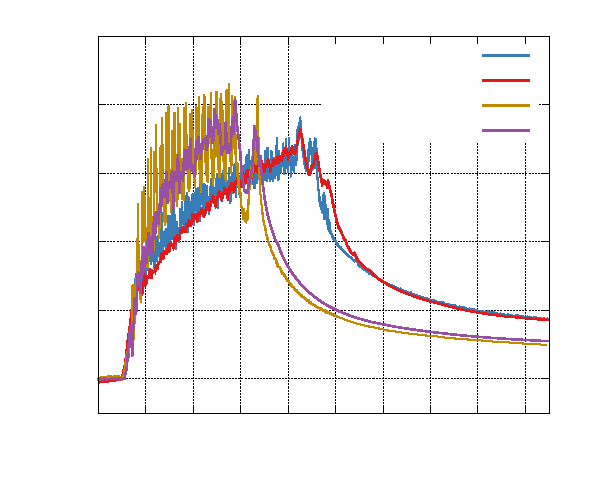
\includegraphics{images/fig-comparison}}%
    \gplfronttext
  \end{picture}%
\endgroup

	}
	\caption{VITA synthetic reconstruction of maximum temperature IR signal compared to experiment IR camera measurement for two H-mode pulses with medium (90271), and high power (92025) input power.}
	\label{fig:Pulses-Comparison}
\end{figure}

\section{Input data}

\subsection{Equilibrium}
	\begin{description}
	\item [Static equilibrium] reading them from equilibrium files in FIESTA or EQDSK formats.
	\item [Sweeping] applies a displacement to the heat load along the divertor target.
	\item [Multiple equilibria] uses several input files for defining a transient plasma load.
\end{description}

\subsection{plasma parameters}



\chapter{Workflow}

\section{Overview}

asdfsafsdaf


\begin{figure}[htb]
	\centering
	%  \vspace{-15mm}
	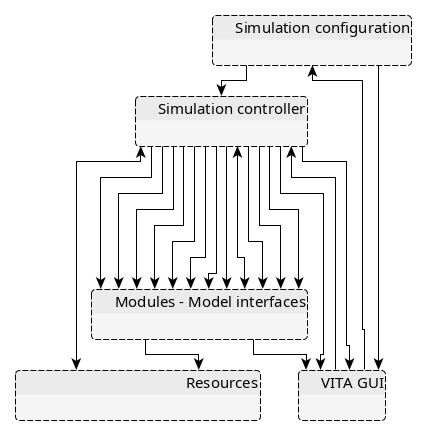
\includegraphics[width=0.60\linewidth]{images/Scheme-top-level}
	\caption{Top level scheme of Vitaproject.}
	\label{fig:scheme-top-level}
\end{figure}

\begin{figure}[htb]
	\centering
	%  \vspace{-15mm}
	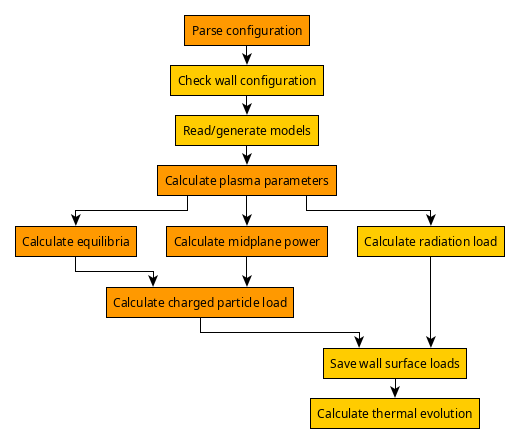
\includegraphics[width=0.90\linewidth]{images/Scheme-simulation-controller}
	\caption{Scheme Vitaproject simulation controller.}
	\label{fig:scheme-top-level}
\end{figure}

\chapter{Theory}

\section{Objectives, formulation and models}
In order to provide the functionality needed, each of the tools tackles one specific phase. As opposed to a typical analysis workflow, the main objective is maximizing the final user's productivity. Their design therefore hides any numerical complexity, and allows their operation using machine and experimental parameters. Several models are provided as a black-box, which is previously validated by analyst experts, but its source code can be inspected, audited, and extended at any time.

The formulation used for this first implementation is based on the thermal equilibrium using the Principle of Virtual Power. The contributions to the power virtual variation, $\delta \dot \Pi$, are calculated from the numerical integration of the following residual equation:

\begin{equation}\label{eq:var_trabajo}
\delta \dot \Pi = \delta \dot \Pi_{capacitance} - \delta \dot \Pi_{external} - \delta \dot \Pi_{conduction} = 0
\end{equation}

Each of the previous contribution terms can be expressed in the reference configuration \cite{Iglesias2015} as:
\begin{eqnarray}
\label{eq:var_potential_th_internal}
\delta \dot \Pi_{capacitance} & = & \int_{\mathcal B} \rho c_p \frac{dT}{dt} \delta T \ dV
\\
\label{eq:var_potential_th_int}
\delta \dot \Pi_{external} & = & \int_{\mathcal \partial B} \bs q \delta T \cdot \bs n \ dS
\\
\label{eq:var_potential_th_conduction}
\delta \dot \Pi_{conduction} & = & \int_{\mathcal B} \left( \bs \kappa \nabla T \right) \cdot \nabla \delta T \ dV
\end{eqnarray}
Where the conductivity tensor $\bs \kappa$ and the specific heat capacity $c_p$, are temperature dependent, $f(T)$, properties of the material. The density $\rho$ is considered constant.


\begin{figure}[htb]
	\centering
	%  \vspace{-15mm}
	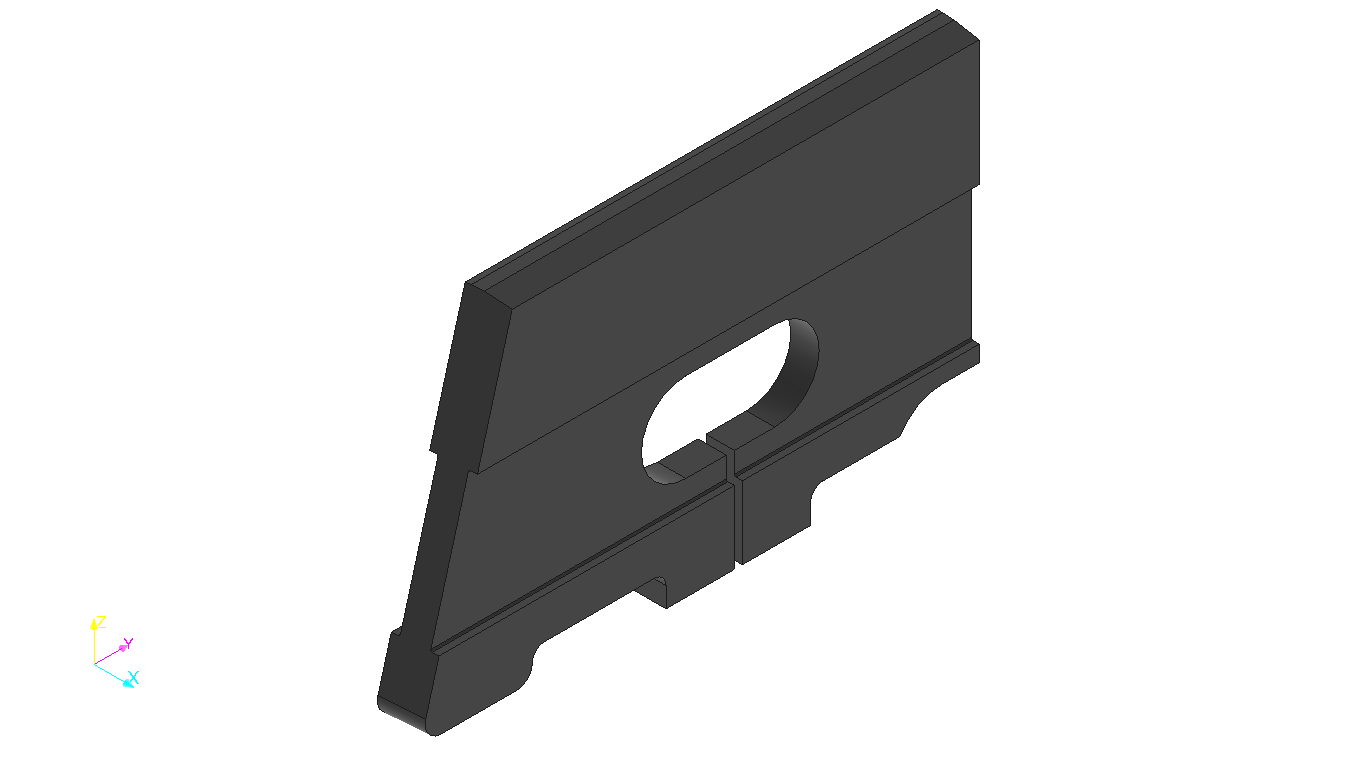
\includegraphics[width=0.48\linewidth,trim={2cm 0 6cm 0},clip]{images/lamella3D-inverse}
	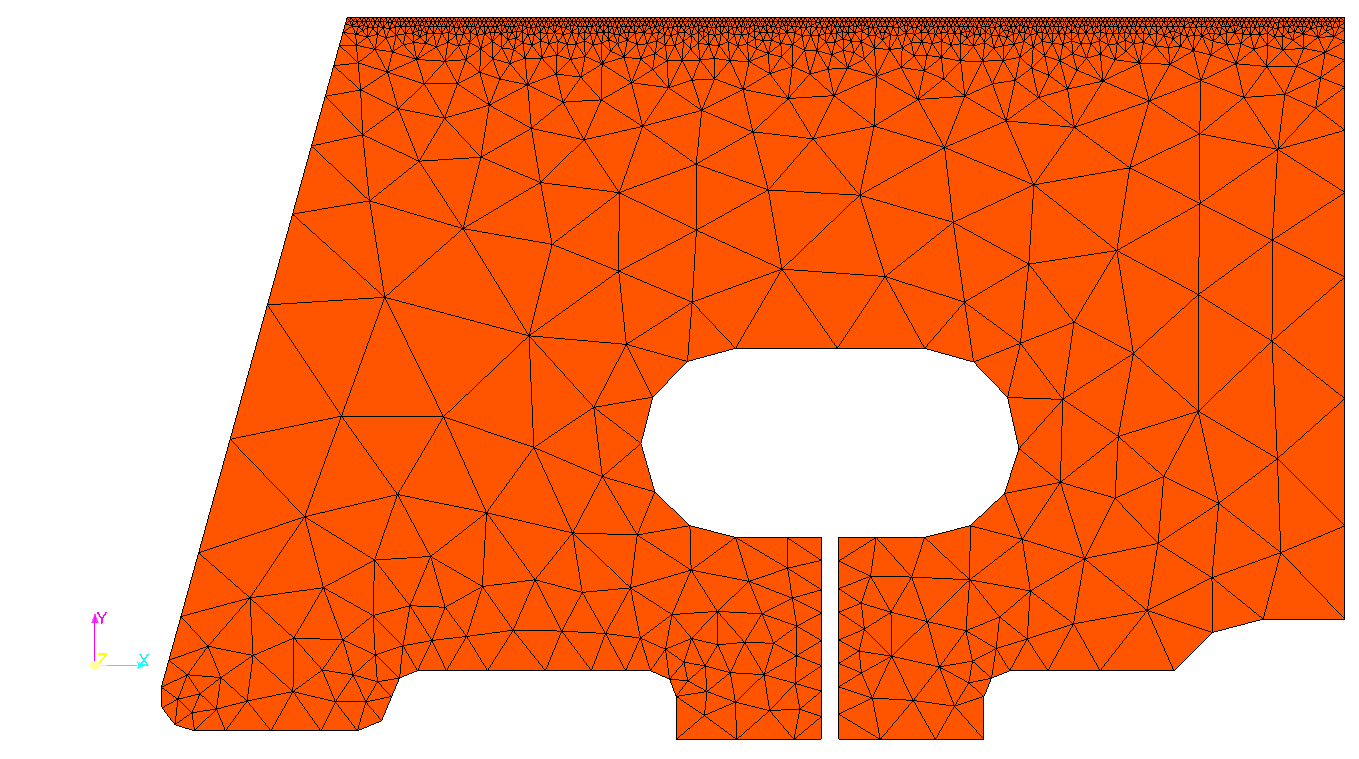
\includegraphics[width=0.40\linewidth]{images/lamella-mesh-inverse}
	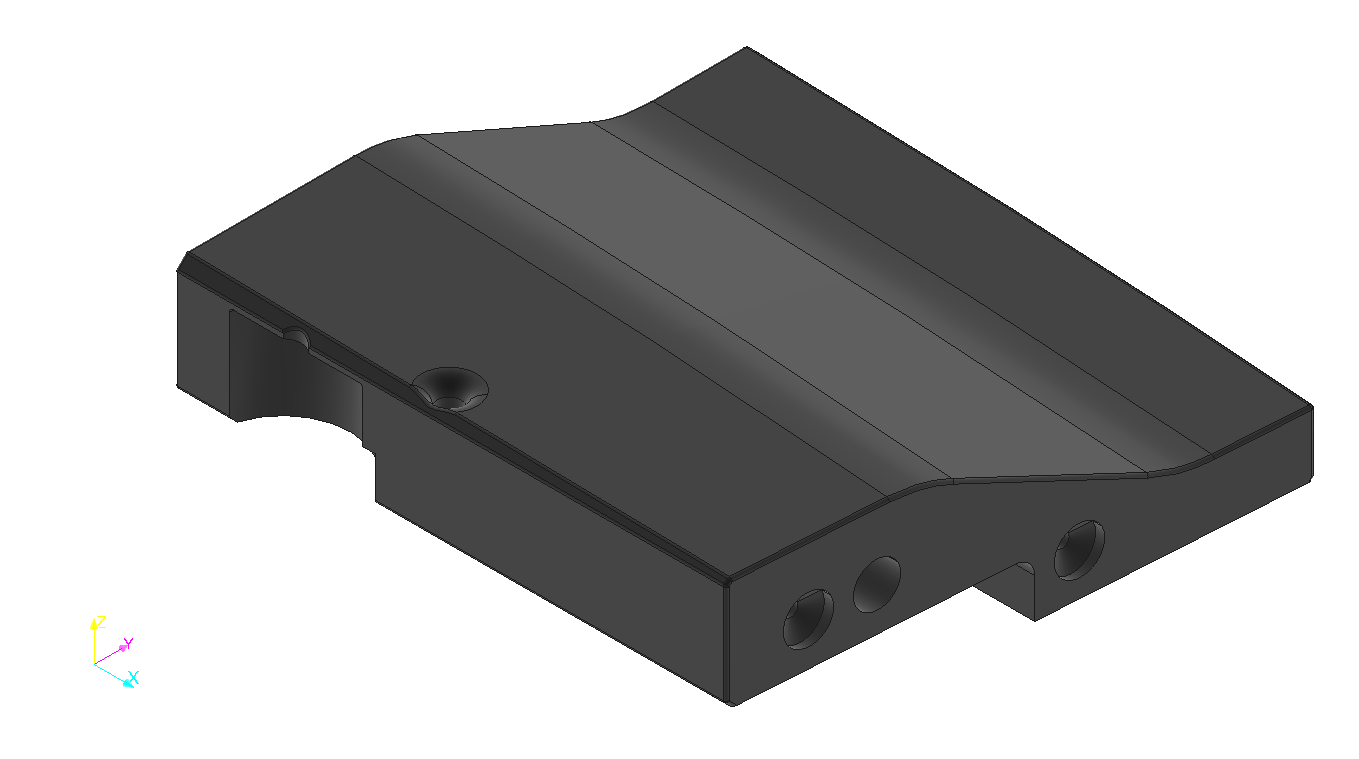
\includegraphics[width=0.50\linewidth]{images/Tile63D-inverse}
	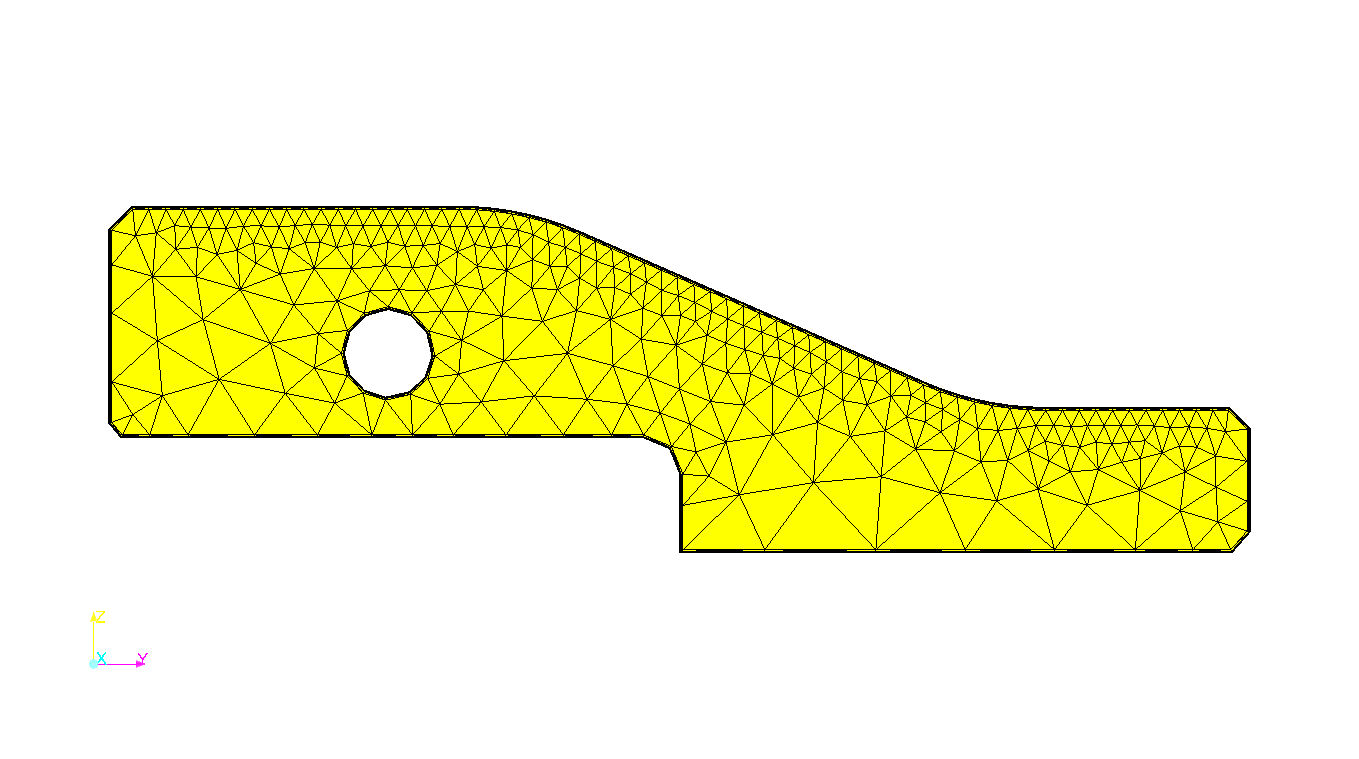
\includegraphics[width=0.48\linewidth]{images/Tile6-mesh-inverse}
	\caption{3D CAD (left) and 2D numerical discretization (right) of divertor components: Tile 5 (top) and tile 6 (bottom).}
	\label{fig:models}
\end{figure}

Fully nonlinear Finite Element (FE) approximations are used for all analyses, with some Galerkin meshfree enhancements \cite{Iglesias2013} when applicable. Several de-featuring levels are applied when speed is a concern. Initial implementation uses 2D models shown in Figure \ref{fig:models}, but design is extensible to 3D in the future. Orthotropic effects, as well as Planck radiation or convection cooling are also foreseen.

Coatings and deposits can be modelled with exact properties, by means of a proper layer formulation which is available for all the applications. Usual parameters for the JET divertor tiles range from 10--\SI{20}{\micro\meter} thickness for the W coating on CFC tiles, to \SI{50}{\micro\meter} node separation in direction normal to the surface for modelling ELMs accurately in bulk W tiles.



\backmatter
% bibliography, glossary and index would go here.
\begin{thebibliography}{00}

\bibitem{Eich2013} T. Eich \textit{et al}, ``Scaling of the tokamak near the scrape-off layer H-mode power width and implications for ITER'', J. Nucl. Mater. 438: S72--S77 (2013).

\bibitem{Riccardo2016} V. Riccardo \textit{et al}, ``Power footprint definition for JET divertor protection'', 22nd International Conference on Plasma Surface Interactions in Controlled Fusion Devices, PSI 22 (2016).

\bibitem{Pamella2015} S. Pamella \textit{et al}, ``Improvements to the Flux Surface Handling Code FLUSH'', Preprint of Paper to be submitted for publication in Fusion Engineering and Design, EUROFUSION WPJET1–PR(15)05.

\bibitem{Jouve2011} M. Jouve \textit{et al},  ``Real-time protection of the 'ITER-like wall at JET' '', Contribution to the Proceedings of the 13th ICALEPCS, p. 1118--1121, ISSN 2226-0358 (2012).

\bibitem{Arnoux2012} G. Arnoux \textit{et al}, ``A Protection System for the JET ITER-like Wall Based on Imaging Diagnostics'', Review of Scientific Instruments, 83(10): 10D727 (2012).

\bibitem{Iglesias2015} D. Iglesias, ``On the application of meshfree methods to the nonlinear dynamics of multibody systems'', Ph.D. Thesis, Universidad Polit\'ecnica de Madrid (2016). \href{https://doi.org/10.20868/UPM.thesis.39121}{https://doi.org/10.20868/UPM.thesis.39121}

\bibitem{Iglesias2013} D. Iglesias \textit{et al}, ``Application of Galerkin meshfree methods to nonlinear thermo-mechanical simulation of solids under extremely high pulsed loading'', Fusion Engineering and Design, 88(9--10): 2744--2747 (2013).

\end{thebibliography}

\end{document}